\chapter{Optimization of steam generating system}
\section{Steam generator subsystem}

In a solar parabolic trough power plant in which intermediate heat-transfer fluid (take oil for instance) is used, heat addition to the working fluid (take water for instance) takes place in three counterflow heat exchangers (steam generator subsystem, SGSS) as shown in fig.~\ref{fig:PTC}. The SGSS is consist of preheater, evaporator, superheater. The flow rates of both oil and water remains the same in the three heat exchangers. 
The water has phase change in the three heat exchangers, from liquid to vapor in the evaporator, however, oil remains liquid. The heat capacity of water in each heat exchanger differs a lot. The heat capacity of oil has no significant difference since no phase change. The heat transfer process is illustrated on fig.~\ref{fig:DeltaTmin}. Large temperature differences exist at the inlets and outlets of the heat exchangers, which makes large entropy production during the entire heat transfer process.


\noindent \begin{figure}[htbp]
\begin{center}
	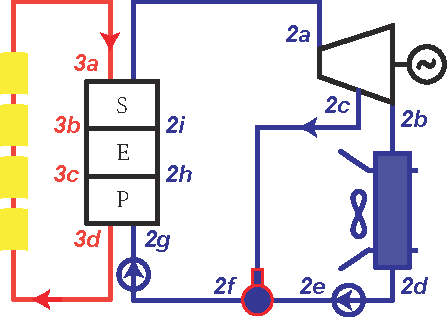
\includegraphics[width = 0.7\columnwidth]{fig/PTC}
	\caption{An typical solar parabolic trough system}
	\label{fig:PTC}
\end{center}
\end{figure}

\noindent \begin{figure}[htbp]
\begin{center}
	\includegraphics[width = 0.7\columnwidth]{fig/DeltaTmin}
	\caption{The steam generating process in countertlow heat exchangers}
	\label{fig:DeltaTmin}
\end{center}
\end{figure}

The heat-transfer fluid at $3a$ represents the solar field outlet temperature and at $3d$, the field return temperature. The difference between these can be reduced by increasing the flow rate of heat-transfer fluid through the field and thus the parasitic pumping power.

Since the heat exchangers must always stay a positive temperature difference for heat transfer, the temperature of oil must always be higher than the temperature of water. On the other hand, the temperature of oil should not be much higher that that of the water. Higher oil temperature leads more heat losses in the solar field hence lower efficiency, more entropy production generated in the heat exchange process. Besides, higher oil temperature brings greater operational risks for the solar system. Setting the appropriate temperature difference between the oil and water is particularly important. The oil temperature must always higher (but no too much higher) than that of the water.

To find out the inlet and outlet temperatures of oil at the solar field, the lowest temperature difference of oil and water is defined as the pinch temperature $\Delta T_{min}$. The temperatures of state points $2h$ and $2i$ are determined by the main pressure of the steam turbine in fig.~\ref{fig:PTC}, and $T_{3b}$ is larger than $T_{3c}$. So state points $3c$ and $2h$, called the pinch point, are set to satisfy the pinch temperature, $T_{3c} - T_{2h} = \Delta T_{min}$. The pinch temperature $\Delta T_{min}$ is usually set to be $10\sim 20\,\mathrm{K}$.
It has to be mentioned that the temperature differences $T_{3d} - T_{2g}$ and $T_{3a} - T_{2j}$ worth attention to be not larger than $\Delta T_{min}$.

However, even with the chosen pinch temperature $\Delta T_{min}$, the temperature difference during the heat exchange process in SGSS is still large due to the phase change of water. Large temperature differences always exists at the inlet/outlet of the exchangers. As shown in fig.~\ref{fig:DeltaT}, it is a tradeoff to choose a mass flow rate of oil ($\dot{m}_3$). $\dot{m}_3$ affects the slope of curve $3a$-$3b$-$3c$-$3d$. A smaller $\dot{m}_3$ leads to a steeper curve, hence a larger $T_{3a} - T_{2j}$. A larger $\dot{m}_3$ leads to a more gentle curve, hence a larger $T_{3d} - T_{2g}$. The heat transfer processes in SGSS always produce large entropy and exergy loss. In this regard, a multi-stage exergy-loss reduction system is put forward.

\noindent \begin{figure}[htbp]
\begin{center}
	\includegraphics[width = 0.7\columnwidth]{fig/DeltaT}
	\caption{An typical solar parabolic trough system}
	\label{fig:DeltaT}
\end{center}
\end{figure}

\section{Multi-stage exergy-loss reduction system}
The reason of large temperature differences of the two curves in fig~\ref{fig:DeltaTmin} is that, $c_p$
\section{Comparison}

In a traditional solar parabolic trough power plant, the potential of exergy loss reduction in the heating process of Rankine cycle is large. There exist large temperature differences between the heat transfer fluid (HTF) and water in the steam generator subsystem (SGSS). In order to reduce the temperature differences, a novel multi-stage exergy-loss reduction system (MERS) with different HTF flows to lower the required HTF temperature is put forward. A flow control strategy of HTF depending on the analytical system model was derived. Energy and exergy efficiency of the MERS was analyzed and compared with the SGSS of traditional solar parabolic trough power plant. Result shows that the MERS can effectively decrease the exergy loss in the heating process, thus the performance of the plant can be improved.


